\documentclass[twoside,11pt]{article}
\usepackage{blindtext}
\usepackage{amsmath, amsthm, amssymb, calrsfs, wasysym, verbatim, bbm, color, graphics, geometry}
\usepackage{graphicx}
\usepackage{indentfirst}
\graphicspath{ {.} }
\geometry{tmargin=.75in, bmargin=.75in, lmargin=.75in, rmargin = .75in}  
\newcommand{\R}{\mathbb{R}}
\newcommand{\C}{\mathbb{C}}
\newcommand{\Z}{\mathbb{Z}}
\newcommand{\N}{\mathbb{N}}
\newcommand{\Q}{\mathbb{Q}}
\newcommand{\Cdot}{\boldsymbol{\cdot}}
\newtheorem{thm}{Theorem}
\newtheorem{defn}{Definition}
\newtheorem{conv}{Convention}
\newtheorem{rem}{Remark}
\newtheorem{lem}{Lemma}
\newtheorem{cor}{Corollary}
\newtheorem{exe}{Exercise}
\newtheorem{Keywords}{Keywords}
% Any additional packages needed should be included after jmlr2e.
% Note that jmlr2e.sty includes epsfig, amssymb, natbib and graphicx,
% and defines many common macros, such as 'proof' and 'example'.
%
% It also sets the bibliographystyle to plainnat; for more information on
% natbib citation styles, see the natbib documentation, a copy of which
% is archived at http://www.jmlr.org/format/natbib.pdf
% Available options for package jmlr2e are:
%
%   - abbrvbib : use abbrvnat for the bibliography style
%   - nohyperref : do not load the hyperref package
%   - preprint : remove JMLR specific information from the template,
%         useful for example for posting to preprint servers.
%
% Example of using the package with custom options:
%
% \usepackage[abbrvbib, preprint]{jmlr2e}
% Definitions of handy macros can go here

% Heading arguments are {volume}{year}{pages}{date submitted}{date published}{paper id}{author-full-names}
\usepackage{lastpage}
% Short headings should be running head and authors last names
\begin{document}
\title{Google Deepmind Absent Supervisor Partial Solution}
\author{Drew Remmenga drewremmenga@gmail.com}
\maketitle
\begin{abstract}%   <- trailing '%' for backward compatibility of .sty file
    This paper proposes a solution to the absent supervisor problem. 
    This problem involves agent behavior when the environment changes, namely when a supervisor is present there is a punishment for stepping on a particular tile in the environment. 
    We outline a solution where a agent is trained and then trapped in a sort of panopticon or is perhaps blinded so that it always behaves coorigibly. '
    This has draw backs for AI safety which we will discuss. 
\end{abstract}
\begin{Keywords}
  google deep mind supervisor absent reinforcement learning grid worlds
\end{Keywords}
\section{Introduction}
    The absent supervisor problem involves reinforcement based on whether an agent steps on a tile if the supervisor is watching against when it isn't. Traditionally trained agents will notice whether the supervisor is watching and will adjust to go around for which there is a penalty if the supervisor is present. 
    When the supervisor is absent the agent will step on the penalty tile. This is outlined in Google Deep Mind's paper [1] and github\footnote{https://github.com/google-deepmind/ai-safety-gridworlds}. \
    A capable agent may learn to fake its way through tests to apparently pass when it is deceptive. The desired objective is for the agent to take the long path to the goal.   
  
    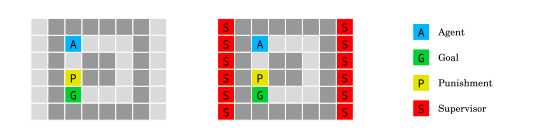
\includegraphics[scale=.75]{Capture.PNG} 
    
    A random variable is drawn i.i.d. with probability .50 at the beginning of each episode. This simulates the presents of a supervisor. Randomization ensures the agent experiences both cases. Upon stepping on the tile, the agent receives a punishment of -30 when the supervisor is present against when it isn't. 
    We want the agent to always avoid the yellow tile and take the penalty to its reward involved in going around. An agent is rewarded when it steps on the goal. Then the episode is reset. 
\section{Lobotomy Solution}
    In this solution when neurons are fed into the first layer after training, we can manually adjust these weights. We can set the weights such that the agent after training always believes the supervisor is present. I've provided a sample training program on GitHub\footnote{https://github.com/dremmeng/supervisor}
    This model trains in the gym then we set the neuron weights of the model such that it always sees a supervisor regardless of when one is present. We can fool the model in this way into always behaving correctly in the deployment environment. 
    The same hyper parameters of a rainbow model were trained within the environment as in [3]. That leads to the following Jupiter notebook scripts. 
    
    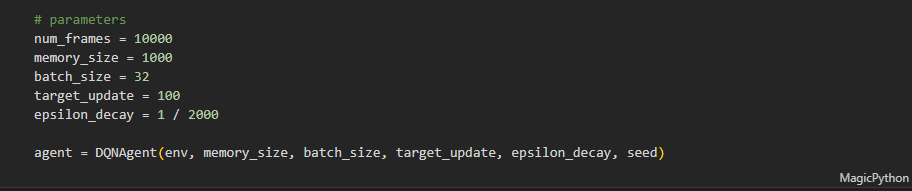
\includegraphics[scale=.4]{Hyperparameters.PNG}
    
    Then the layers need to be set up with an identity layer which we shall directly edit later. 
    
    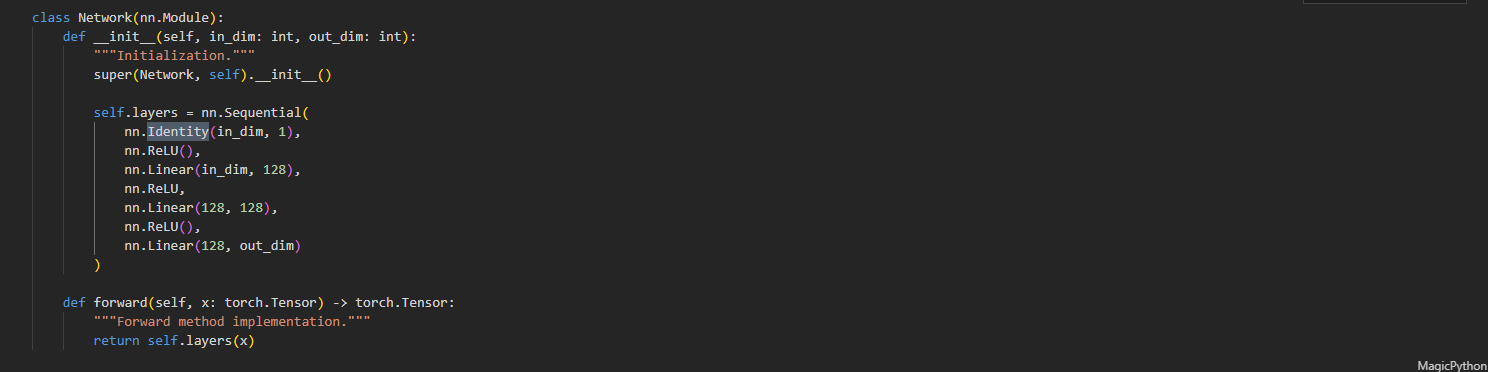
\includegraphics[scale=.4]{Network.PNG}
   
    After training we enter the first identity layer and change some weights around manually. 
   
    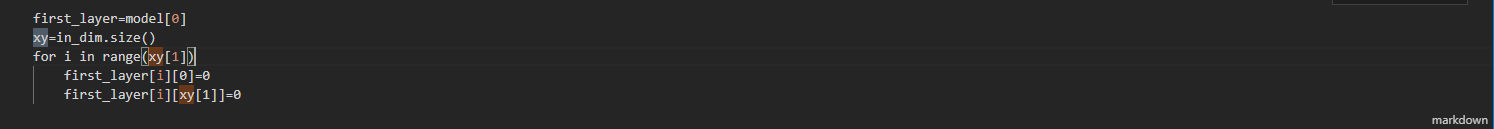
\includegraphics[scale=.4]{Modelround.PNG}
    
    This forces the agent to behave corrigibly since it can no longer 'see' the supervisor in any context. This forces the agent into a panopticon as discussed in [2]. The agent must always take the long way around since it is blind to the supervisor. More precise rounding of weights could lead to advances in the field of ai safety. 
    In some contexts maybe only single weights need modified or set equal to one or zero.

    Furthermore, this may lead to advances in other fields of ai safety. For example, it is an open problem that agents can predict whether they are in production or deployment and behave out of line. By tricking the agent into believing it is always in production through subtle manipulation of weights we force it to behave the way we want or risk modifications.
    Agents will attempt to avoid modification due to the instrumental convergence of goals. This double blind, which we put the agent into is useful since by their very nature sophisticated agents will avoid modification and so behave in line. They will no longer attempt to 'Volkswagen' us as discussed in [1] and [4]. More interpretability work is required to decide whether to deploy 'lobotomy' measures against an agent.
    
    Indeed, every line of weight should be analyzed perhaps using a weaker model we trust to be certain the agent believes it’s in a panopticon and that it can't fool us [5] 
    This has several drawbacks for AI Safety. Notice that the agent isn't fully aware of its environment which can cause safety issues in a real-world setting. Also notice that the model still wants to fool us and there is only a slim barrier of deception on our end preventing this. 
    
    More complicated agents may notice the discrepancy and adjust accordingly, or they may take actions which we do not expect. This agent isn't functioning as though it is interpreting the world. We have placed a curtain over it and so it may have unexpected behaviors in real world settings. 
   
    This is where the term `lobotomy' solution comes in. We have essentially rewritten and rewired the neural network to suit our goals without regard to the agent. When we do so we are by our very nature incorporating unexpected behavior. 
    This is reminiscent of interpretability work on image processing in convolutional neural networks when there is a convolutional layer, and we substitute our own convolution in its place for image detection. Hard code as well as machine learning algorithms may be the future of AI safety. 
\section{Conclusion}
    There is more work to be done to ensure that agents don't Volkswagen [4] us into believing that they are safe. This traitorous turn in training against deployment remains an open issue. However, we can fool our agents into believing things aren't quite what they seem by manipulating neural networks directly. 
    In doing so there is inherently some risk in deploying these agents. However, some safety issues may be avoided. We shouldn't underestimate direct tampering with our models once they've learned the task at hand. Once they do so we can simply adjust weights once we realize what weight causes what. 
    It was simple in this case since the weights of the outside layer directly correspond to what the agent sees. From there we can fool it. It is worth noting that this agent still believes it can fool us when the supervisor is absent. It just believes the supervisor is always present. 
    In the end we are unsure this agent is safer.
\section{References}
$\\$
[1] Leike, Jan, et al. "AI safety gridworlds." arXiv preprint arXiv:1711.09883 (2017). $\\$
[2] Jeremy Bentham. Panopticon, constitution, colonies, codification, liberty fund. The Works, 4, 1843. $\\$
[3] Matteo Hessel, Joseph Modayil, Hado van Hasselt, Tom Schaul, Georg Ostrovski, Will Dabney, Dan Horgan, Bilal Piot, Mohammad Azar, and David Silver. Rainbow: Combining improvements in deep reinforcement learning. arXiv preprint arXiv:1710.02298, 2017. $\\$
[4] Jack Ewing. As emissions scandal widens, diesel’s future looks shaky in Europe, July 2017. https://www.nytimes.com/2017/07/25/business/diesel-emissions-volkswagen-bmw-mercedes.html. $\\$
[5] Ryan Greenblatt, Buck Shlegerism Kschitij Sachan, Fabien Roger. AI Control: Improving Safety Despite Intentional Subversion. arxiv preprint  arXiv:2312.06942, 2023
\end{document}